%%%%%%%%%%%%%%%%%%%%%%%%%%%%%%%%%%%%%%%%%%%%%%%%%%%%%%
\chapter{Experimental design}
\label{experimental_design}
\graphicspath{{chapter_03/figures}{chapter_03/tables}}
%%%%%%%%%%%%%%%%%%%%%%%%%%%%%%%%%%%%%%%%%%%%%%%%%%%%%%


This chapter articulates the sequential experimental strategy designed to address the research questions presented in Chapter \ref{general_introduction} and provide the proof of concept for medium-range predictions of areas at risk of flash floods across a continuous global domain. The strategy follows a three-component approach, where each component builds upon the findings of the previous one (Figure \ref{fig:workflow_dataflow}). 

\begin{figure}[htbp]
\centering
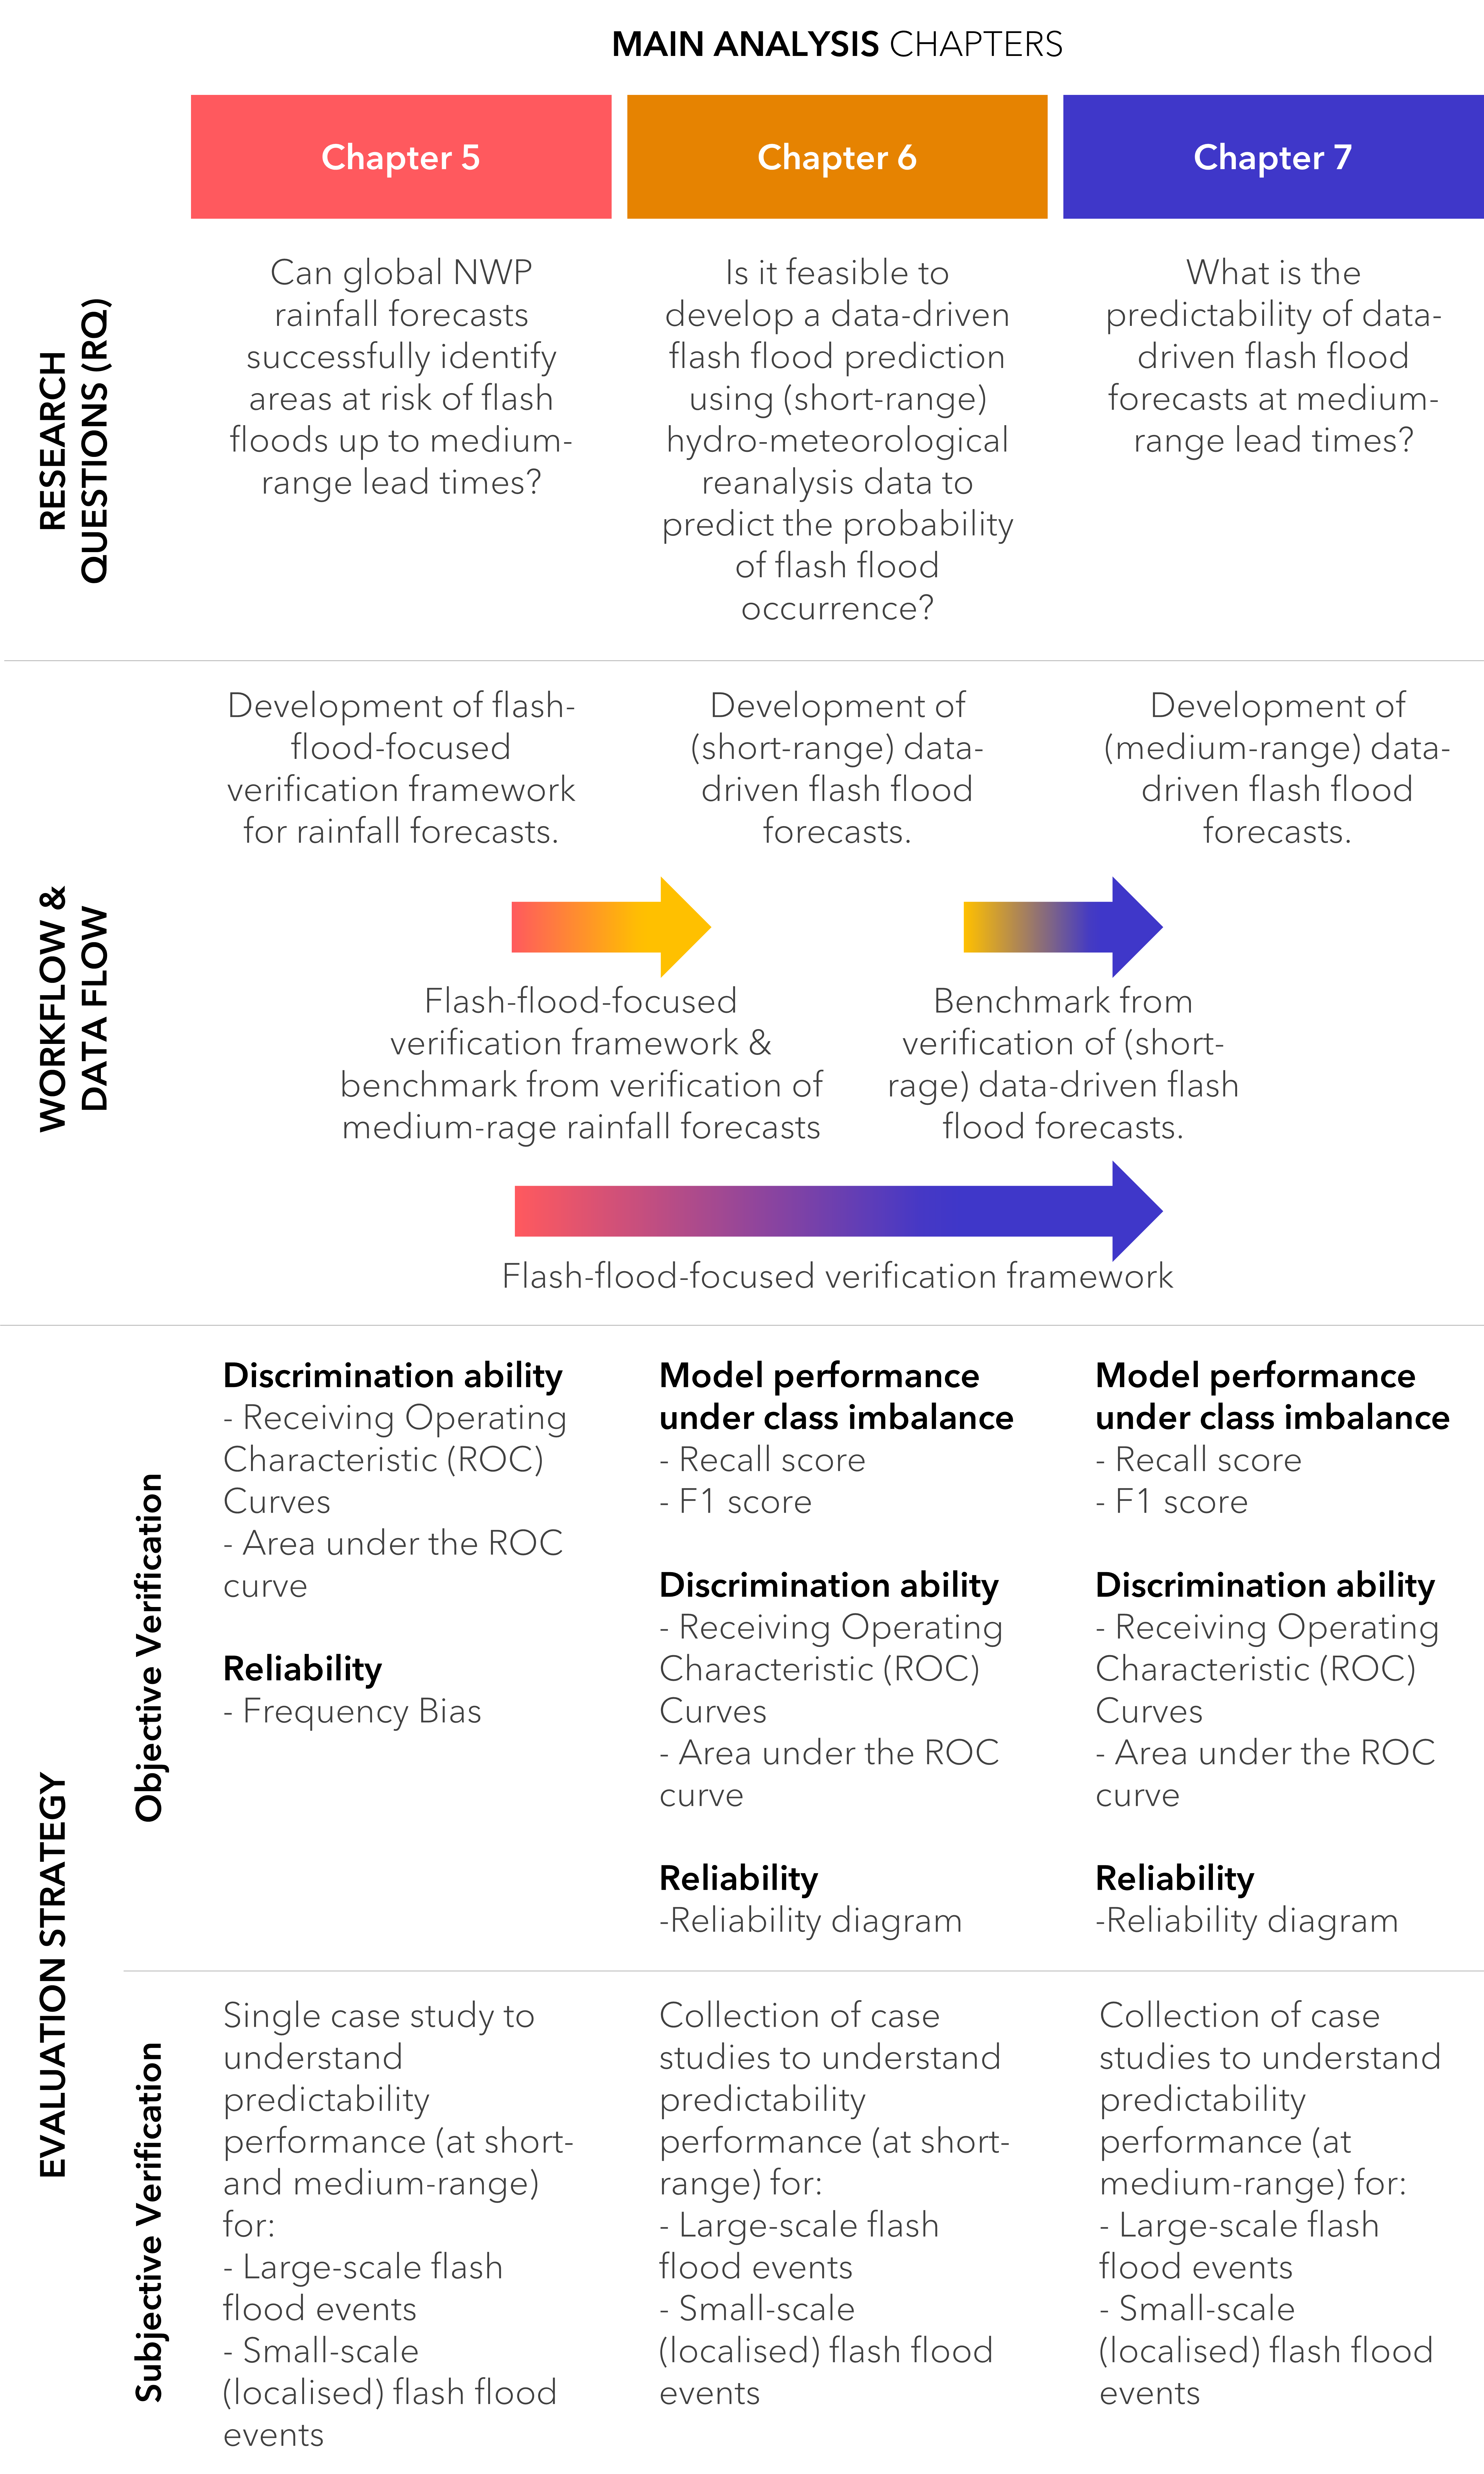
\includegraphics[width=\textwidth]{workflow_dataflow.png}
\caption{\textbf{Overview of the experimental design across the "Main Analysis" chapters (5 to 7).} The infographic delineates the research questions addressed in each chapter, the workflow of data flow across the chapters, and the adopted evaluation strategies to assess the performance of global NWP rainfall forecasts and data-driven flash flood predictions in identifying areas at risk of flash floods.}
\label{fig:workflow_dataflow}
\end{figure}

The \marginpara{First methodological component (addressing RQ1): development of a flash-flood-focused verification framework to assess predictions of areas at risk of flash flood} first methodological component addresses the challenge that high-quality rainfall forecasts do not necessarily translate directly to accurate flash flood predictions. It therefore assesses the capability of medium-range global rainfall forecasts to identify areas at risk of flash floods up to medium-range lead times by proposing a flash-flood-focused rainfall verification framework. This initial verification is essential as it establishes the baseline predictive capacity of rainfall predictions from state-of-the-art global NWP models to identify areas at risk of flash flood risk.

The \marginpara{Second methodological component (addressing RQ2): development of short-range data-driven hydro-meteorological predictions of areas at risk of flash floods - Regional prototype and global transferability assessment} second methodological component develops a data-driven framework to identify areas at risk of flash floods over the CONUS. This data-driven approach represents a departure from traditional physically based hydrological modelling of flash floods, which often struggle with computational demands and parameter uncertainty. This second methodological component also runs a sensitivity analysis to assess which data strategy would be the most appropriate for the global extension of the regional training, so predictions over a continuous global domain can be computed.

The \marginpara{Third methodological component (addressing RQ3): development of medium-range data-driven hydro-meteorological predictions of areas at risk of flash floods - Regional and global prototype} third methodological component extends the application of the data-driven model to medium-range forecasts, enabling the assessment of flash flood predictability beyond typical short-range (day 0) predictions. This component synthesises the findings from the previous two methods, applying the data-driven framework developed in the second stage to longer-range forecast data and the verification framework developed in the first stage of the analysis to evaluate how predictive skill for flash flooding decays with increasing lead times. This evaluation is crucial for understanding the temporal limitations of actionable flash flood predictions.

The following sections will detail each methodological component, including data sources, processing techniques, model development procedures, and verification frameworks adopted in this study. 

data sources (which component relates to), make it look like I thought it all together.

ADD THE CROSS REFERENCING ALL OVER THE THESIS TO AVOID REPETITIONS OR TOO MUCH DETAIL.


%%%%%%%%%%%%%%%%%%%%%%%%%%%%%%%%%%%%%%%%%%%%%%%%%%%%%%%%%%%%%%%%%%%%%%%%%%%%
\section{Flash-flood-focused verification framework}

\begin{figure}[htbp]
\centering
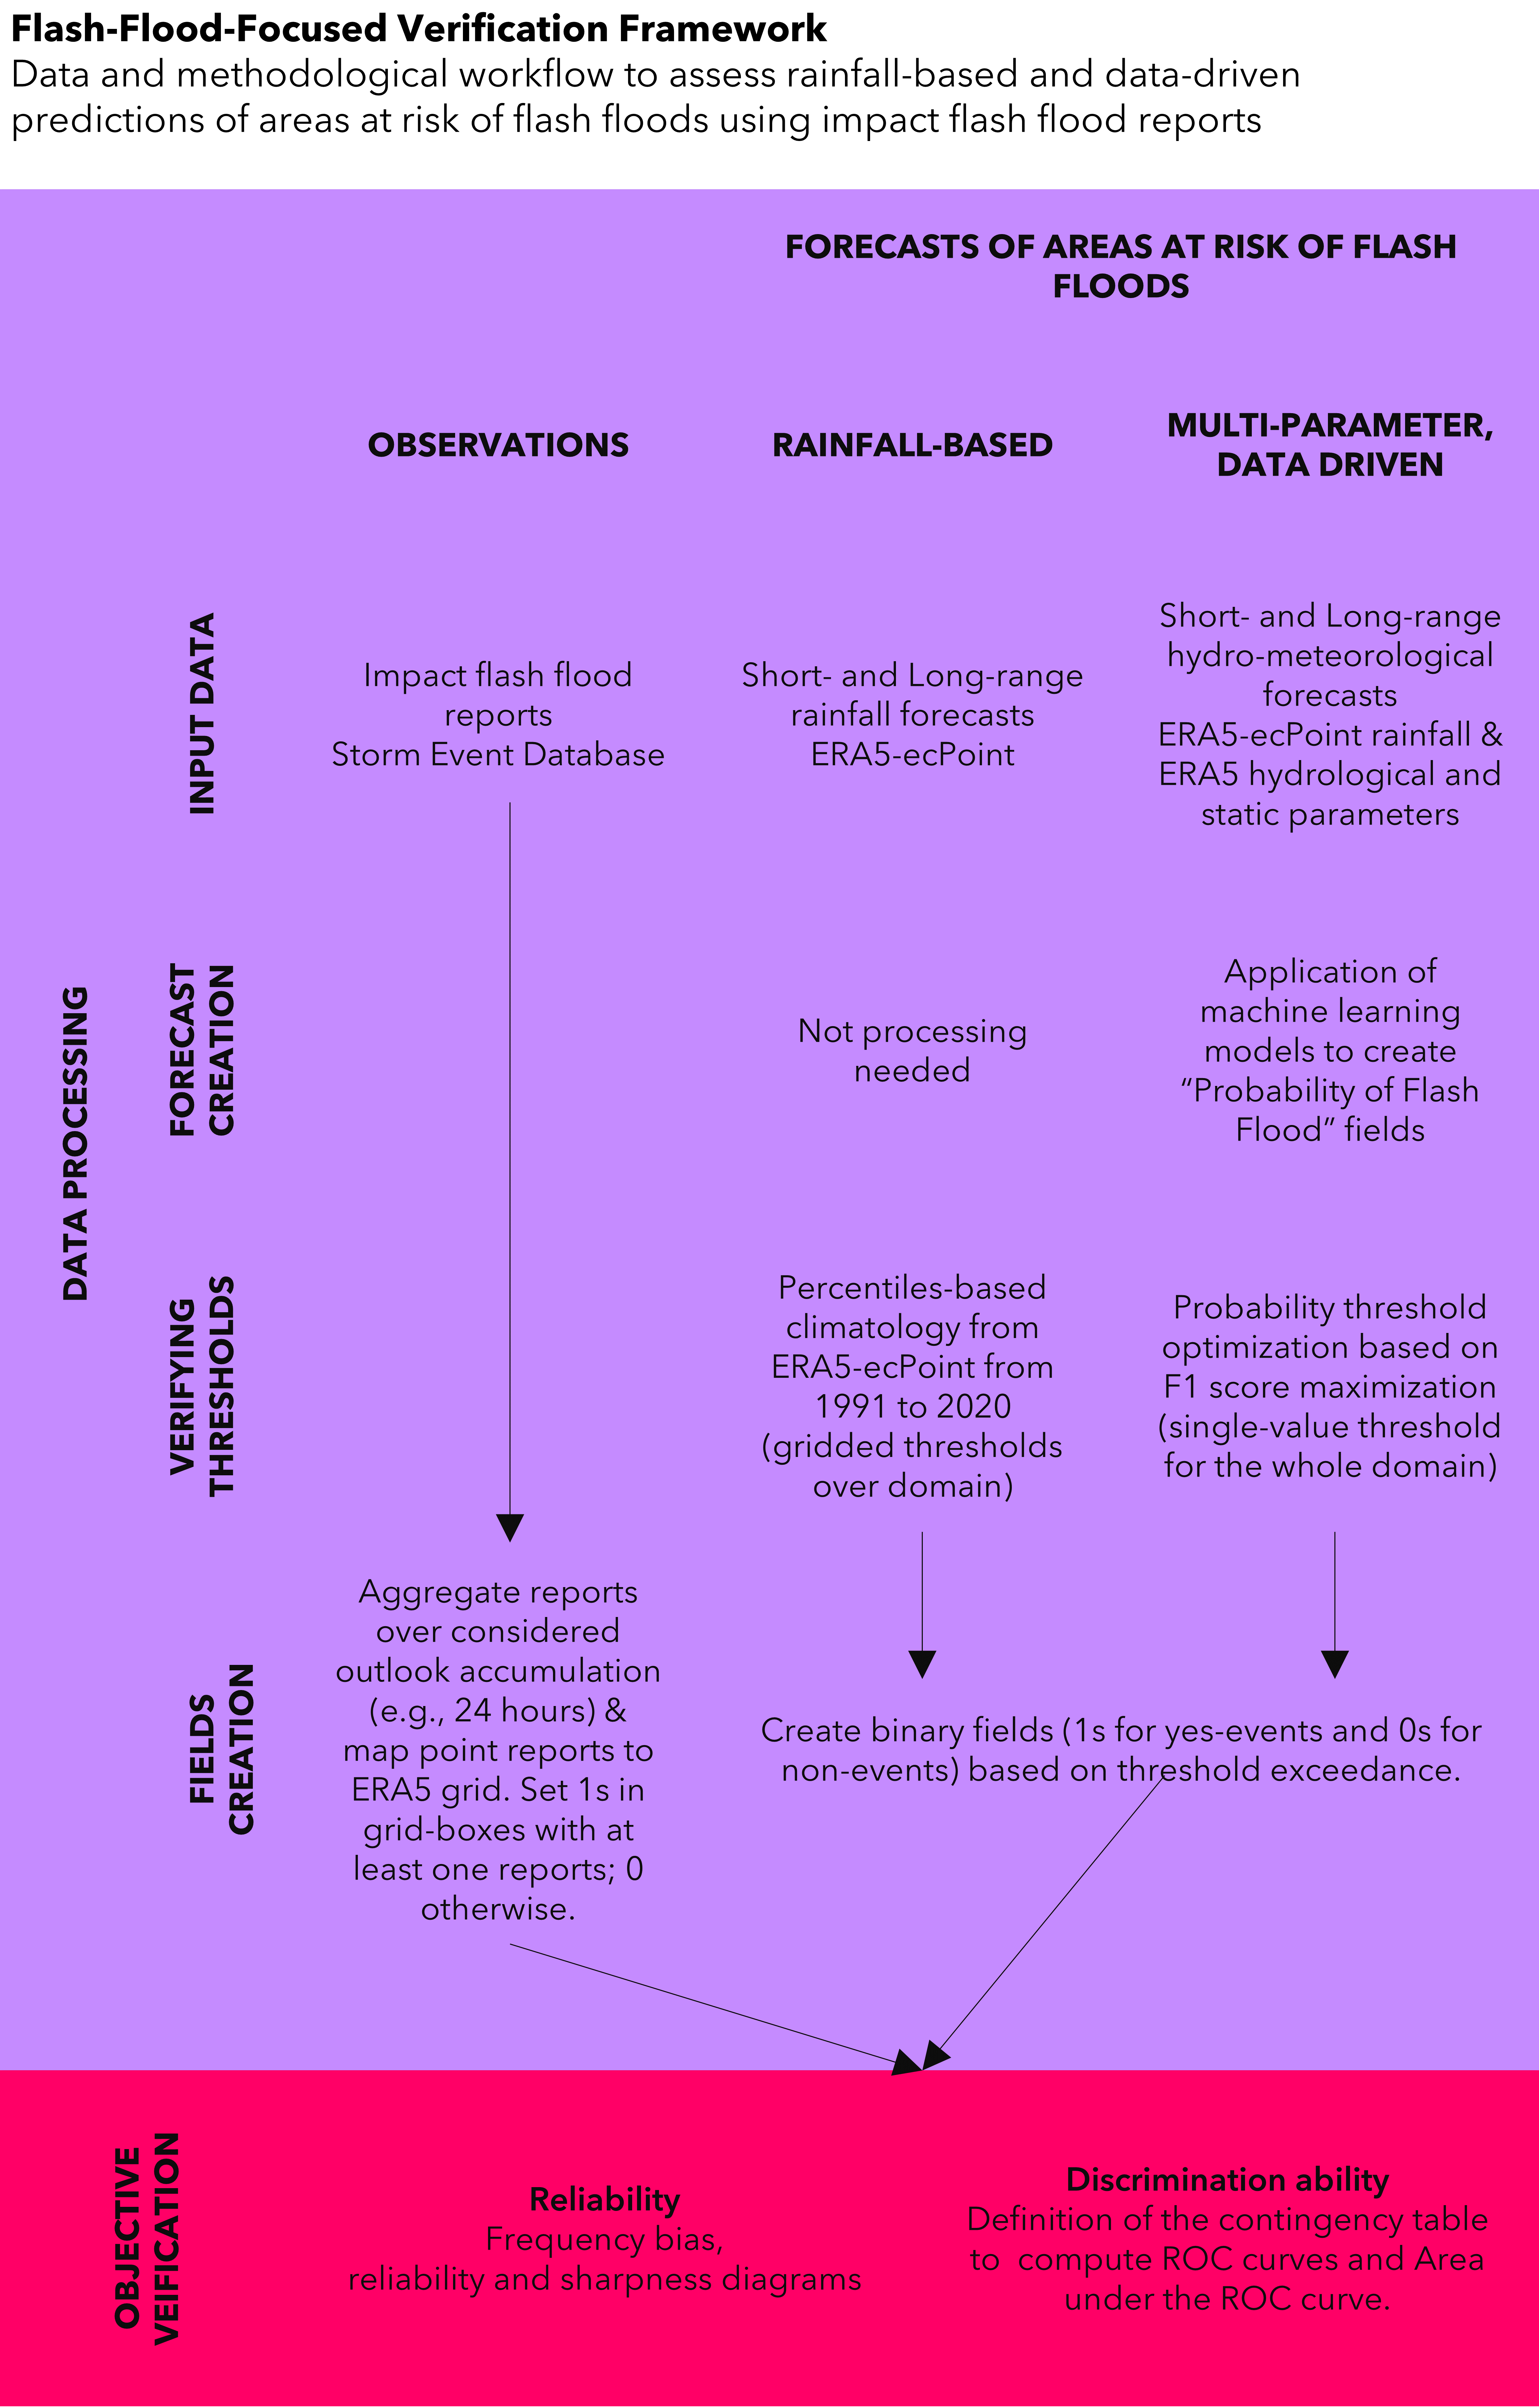
\includegraphics[width=\textwidth]{workflow_verif_framework.png}
\caption{\textbf{Workflow for flash-flood-focused verification framework.} Data and methodological framework to assess predictions of areas at risk of flash floods using impact flash flood reports.}
\label{fig:workflow_verif_framework}
\end{figure}

\subsection{What observational data are required for flash flood verification?}

The selection of appropriate observational data constitutes a critical foundation for any verification framework. This study utilises the Storm Events Database, maintained by the National Oceanic and Atmospheric Administration (NOAA), as the primary source of flash flood observations across the Continental United States (CONUS). This database represents the most comprehensive and systematically maintained record of flash flood impacts available at continental scale, containing detailed spatio-temporal information for events from 1950 to the present (purple area in Figure \ref{fig:workflow_verif_framework}).

The choice of an impact-based database rather than hydrological measurements reflects the fundamental nature of flash floods as localised phenomena occurring predominantly in ungauged catchments. Traditional gauge-based observations fail to capture the majority of flash flood events due to their sparse spatial distribution and the rapid onset characteristics of these events. Impact databases, whilst subject to reporting biases, provide a more feasible approach for continental-scale verification where the installation and maintenance of dense observational networks remains economically and logistically prohibitive.

The Storm Events Database offers several advantages that justify its selection. First, it provides consistent reporting standards across all US states, enabling uniform analysis across diverse hydro-climatic regions. Second, each report includes precise geolocation data, essential for grid-based verification approaches. Third, the database undergoes quality control procedures by NOAA, reducing, though not eliminating, reporting inconsistencies that might be present in other databases such as ESWD (with clear reporting biases over Germany). These characteristics make it the most suitable dataset for establishing a robust verification framework, acknowledging that similar approaches could be applied to other regional databases such as the European Severe Weather Database or global repositories like EM-DAT and Desinventar, each with their specific limitations and biases.


\subsection{Why using ERA5 and ERA5-ecPoint data in the development of predictions of areas at risk of flash floods?}

The ERA5 dataset was selected in this thesis as it provides a long-term (from the 1950s to the present), high-quality reconstruction of hydro-meteorological fields over a continuous global domain \citep{Hersbach_2020}. Thus, the short-range forecasts (up to day 0, and also known as \textit{reanalysis}) provide a good dataset for the training of the data-driven predictions. While ERA5 provides a consistent dataset for training over space and time, its coarse resolution makes raw ERA5's rainfall estimates not appropriate for flash flood applications as localised rainfall peaks tend to be underestimated, and severely underestimated in the case of isolated convection. For this reason, the rainfall estimates used for training and verification come from the post-processed ERA5 rainfall estimates with the ecPoint methodology, which provides a probabilistic distribution of how the localised extreme rainfall estimates might be. A more detailed description of the post-processing methodology and the quality of the ecPoint rainfall forecasts can be found in section \ref{ecpoint_rainfall}.

Regarding the longer-range forecasts used to create the medium-range predictions of areas at risk of flash floods, it is common practice to fine-tune the training done with lower-resolution datasets (such as ERA5, at 31 km) to the higher resolution of typically used forecasting systems (such as ECMWF's IFS, at 9 km). In the field of data-driven weather forecasts, this is done in the AIFS, which is trained over ERA5 and fine-tuned over the operational analysis at 9 km to obtain forecasts with a spatial resolution of \sim25 km  \citep{Lang_2024}. This approach was not adopted in this thesis as it would introduce uncertainties in the forecasting chain related to such fine-tuning that would be difficult to dissociate from uncertainties due to the prediction of the hazard itself. Hence, the long-range forecasts from ERA5 and corresponding ecPoint post-processed rainfall estimates were used in this thesis. Even though this approach means creating a low-resolution prototype for flash flood prediction (as the medium-range forecasts remain provided at 31 km resolution), the forecast uncertainties presented in this thesis remain detached from fine-tuning processes and can be related primarily to the physical processes that generate flash floods and the data used to create the short- and medium-range forecats.

\subsection{How should flash flood observations be processed for grid-based verification?}

The transformation of point-based impact reports into gridded observational fields requires careful consideration of spatial and temporal aggregation methods. This study implements a systematic approach aligned with established severe weather verification methodologies \citep{Tsonevsky_2018, Pillosu_2024}.

Each flash flood report undergoes temporal aggregation to match the 24-hour accumulation periods of the forecast products, beginning at 00 UTC. This alignment ensures consistent comparison between observations and predictions whilst acknowledging that flash floods may occur at any time within the accumulation window. The choice of 24-hour periods balances the need for sufficient temporal resolution with the practical constraints of forecast product availability and the typical duration of flash flood events.

Spatial assignment of reports to the ERA5 grid (approximately 31 km resolution) employs a nearest-neighbour approach for point reports and polygon inclusion for events with spatial extent. Given the relatively coarse resolution of ERA5 grid boxes compared to typical flash flood scales, additional spatial expansion techniques commonly used in convective-scale verification prove unnecessary. The resulting gridded fields preserve information about event frequency within each grid box, enabling more nuanced verification than binary occurrence fields.
This processing approach addresses the fundamental challenge of scale mismatch between localised flash flood events and gridded forecast products. The methodology provides a reproducible framework applicable to other grid resolutions and accumulation periods, with detailed implementation provided in chapter \ref{flash_flood_focused_verification_framework}.


\subsection{What verification thresholds enable meaningful assessment of flash flood predictions?}

The establishment of appropriate verification thresholds represents a critical methodological decision that directly influences all subsequent analyses. 

For rainfall-based predictions, thresholds must reflect the precipitation amounts capable of generating flash floods across diverse hydro-climatic conditions. In the absence of comprehensive observational networks capturing extreme precipitation at flash flood scales, this study develops a novel approach using ERA5-ecPoint rainfall estimates. ERA5-ecPoint provides bias-corrected, post-processed rainfall estimates that better represent point-scale extremes compared to raw ERA5 data \citep{Pillosu_2025a}. A 30-year climatology (1991-2020) following WMO standards enables the derivation of location-specific rainfall thresholds corresponding to various return periods. This approach captures the spatial heterogeneity of flash flood susceptibility, recognising that identical rainfall amounts may produce vastly different impacts depending on local conditions. The selection of multiple threshold percentiles allows examination of forecast performance across the full spectrum of flash flood severity. Lower percentiles capture more frequent, lower-impact events, whilst higher percentiles focus on rare, catastrophic floods. This multi-threshold approach provides insights into how forecast skill varies with event rarity and severity, essential information for operational implementation where different stakeholders may have varying risk tolerances.

For hydro-meteorological, data-driven predictions, the verifying thresholds emerge directly from the machine learning algorithms that generated the predictions themselves, applying an optimisation that establishes the probability values that maximise the F1-score when converting a probabilistic prediction into a yes- or non-event. This data-driven threshold selection represents a departure from traditional approaches based, for example, on assumptions about the severity of the triggering events (as done for the rainfall-based forecasts). It instead allows the data-driven models itself to identify optimal decision boundaries to convert the probabilistic forecasts into a yes- or a non-event. As such, the thresholds will be defined based on the frequency of the yes-events in the observational datasets, delivering smaller verifying thresholds for rarer events. 


\subsection{Which verification metrics provide a comprehensive assessment of forecast quality?}

The verification framework employs a suite of metrics designed to evaluate different aspects of forecast performance, recognising that no single metric can fully characterise prediction quality for rare events like flash floods (pink area in Figure \ref{fig:workflow_verif_framework}). The selection of metrics addresses two primary forecast attributes: reliability and discrimination ability.

Reliability assessment examines whether predicted probabilities accurately reflect observed frequencies. The frequency bias provides an aggregate measure of systematic over- or under-prediction, whilst reliability diagrams offer detailed insights into calibration across the full probability spectrum. These metrics prove particularly valuable for understanding how well forecast systems capture the climatological frequency of flash floods, a fundamental requirement for risk-based decision making.

Discrimination ability quantifies the forecast system's capacity to distinguish between flood and non-flood situations. The Area Under the Receiver Operating Characteristic curve (AROC) provides a threshold-independent summary measure, whilst the full ROC curve reveals performance trade-offs at different probability thresholds. For rare event prediction, discrimination ability often represents the primary challenge, as models must identify subtle signals preceding infrequent occurrences.

The choice of probabilistic metrics reflects the inherent uncertainty in flash flood prediction and the need for risk-based decision frameworks in operational contexts. Deterministic metrics prove less suitable given the rarity of events and the importance of capturing forecast uncertainty. Detailed mathematical formulations and computational procedures are provided in the relevant analysis chapters.

%%%%%%%%%%%%%%%%%%%%%%%%%%%%%%%%%%%%%%%%%%%%%%%%%%%%%%%%%%%%%%%%%%%%%%%%%%%%%%%%%
\section{Development of data-driven predictions of areas at risk of flash floods}


\subsection{How can data-driven models address the extreme class imbalance in flash flood data?}

The development of data-driven flash flood prediction models must confront the fundamental challenge of extreme class imbalance, with flash flood events representing approximately 0.2\% of the observational dataset. This imbalance poses significant challenges for machine learning algorithms, which may converge to trivial solutions that never predict positive events.

This study adopts ensemble learning techniques as the primary strategy for addressing class imbalance. Unlike data-level approaches that modify the training dataset through over- or under-sampling, ensemble methods preserve the original data distribution whilst improving minority class detection through algorithmic diversity. This choice reflects a deliberate decision to maintain the integrity of the observational dataset, avoiding the introduction of synthetic samples or the loss of potentially informative negative examples.

The experimental design incorporates multiple ensemble algorithms, including Random Forest, Gradient Boosting variants (XGBoost, LightGBM, CatBoost), neural networks, and ensemble stacking. Each algorithm offers different mechanisms for handling imbalanced datasets, from the inherent bootstrap sampling in Random Forest to the sequential error correction in boosting methods. This diversity enables a comprehensive assessment of which algorithmic approaches best suit the flash flood prediction challenge.


\subsection{What training strategy ensures robust assessment of model performance when working with an extremely imbalanced dataset?}

The validation framework employs nested cross-validation with hyperparameter optimisation to provide unbiased performance estimates whilst maximising model performance. This approach addresses the risk of overfitting inherent in machine learning applications to imbalanced datasets.

The outer cross-validation loop uses stratified k-fold splitting to ensure representative class distributions in all data partitions. Within each outer fold, an inner optimisation loop identifies optimal hyperparameters using Bayesian optimisation via the Optuna framework. This nested structure prevents information leakage between hyperparameter selection and performance evaluation, providing realistic estimates of operational performance.
The choice of AROC as the optimisation metric during hyperparameter tuning reflects its suitability for imbalanced classification and alignment with the verification framework. Alternative metrics such as F1-score prove less suitable due to their dependence on classification thresholds and potential instability with extreme class imbalance.

Repeated evaluation across multiple cross-validation folds quantifies performance variability and identifies potential instabilities in model training. This comprehensive validation approach ensures that reported performance metrics reflect genuine predictive capability rather than fortunate data splits or overfitting to specific training samples. Implementation details and computational considerations are discussed in Chapter \ref{feasibility_PoFF}.
